\section{Route Designer Web Page}

For this sprint, a route designer web page was desired. Its functionality should include a map where users could create and modify routes, as well as a user login system to restrict access to a user's own routes.

\subsection{Graphical User Interface}
\label{sub:sprint1-web-gui}

A simple user interface was designed. An initial mock-up can be seen in \autoref{fig:sprint1-web-ui}, which shows the desired layout of the route planner display. The general philosophy was to keep the layout consistent on all pages. As such, the title and the menu will be at the same position on all views, though the menu options will change depending on the permissions of the user, in this case whether the user is logged in or not.

\begin{figure}[ht]
 \caption{Web UI Mock up}
 \label{fig:sprint1-web-ui}
 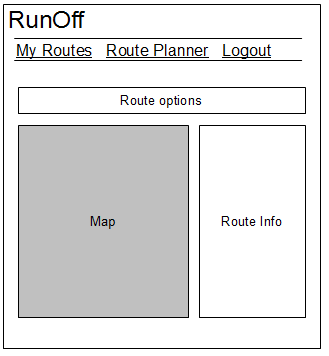
\includegraphics[scale=1]{img/webmockup1.png}
\end{figure}

Four views, which should constitute an \ac{MVP}, were planned for this sprint:
\begin{itemize}
 \item {Route Designer} (Only available when logged in)
 \item {Route Overview} (Only available when logged in)
 \item {User Registration}
 \item {User Log In}
\end{itemize}

The route overview should be a simple listing of the routes the current user has created, with a summary of the information available for that route, as well as a link to modify each route. The registration and log in views should be simple \ac{HTML} forms.

The route planner is where most of the work should be done. The planner should display a map, and the following controls on the map:

\begin{itemize}
 \item Clicking the map should add a waypoint
 \item Clicking and dragging a waypoint should move it
 \item Right-clicking a waypoint should delete it
\end{itemize}

After each of these actions has been performed, a route should be created, snapping the route to paths and pavements, as well as allowing users to see useful information, such as the total distance and topography of the route.

Additionally, the planner should expose various controls separate from the map itself, including the ability to name the route, mark it as a round-trip (Using the first waypoint as both start and end of the route) as well as submitting the route and saving it on the server.

\subsection{Database Model}

The route planner needed a database to store the routes for each user. The database design can be seen in \autoref{fig:sprint1-db-model}. This simple design allows for multiple users to store a number of routes which each have several waypoints. The index column in the \texttt{Waypoint} table is the waypoint ``number'' within the route, and this design allows sorting the waypoints correctly already at the time where they are retrieved from the database.

\begin{figure}[ht]
 \caption{Sprint 1 Database Model}
 \label{fig:sprint1-db-model}
 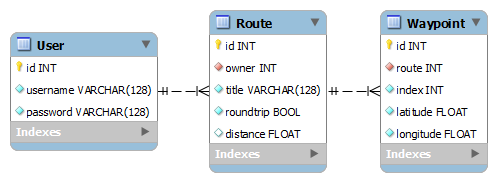
\includegraphics[scale=0.5]{img/sprint1db.png}
\end{figure}

The decision to use a boolean on the \texttt{Route} to denote whether or not the route is a round-trip, rather than saving two copies of the first waypoint with different index values, was made partly because it results ion less database entries, but the primary reason was that it made it easier to correctly load the settings of a previously saved route, should the user desire to edit it. Distance is allowed to be \texttt{null} for a route, for the reason that a user might save a route with less than two waypoints, or waypoints which might not be reachable from each other with the intent to fix it later.

\subsection{Implementation}

Implementing the web page was done in two parts, the server and client.

\subsubsection{Server Implementation}

The server was implemented in the Django\cite{djangoproject}, a web framework for the Python programming language. We made use of several of the features of Django, to ease the implementation of the previously mentioned design. An example of this, is Django's \ac{ORM}, which was used to implement the database, removing any need to write database code directly. As such, the \texttt{Route} table seen in \autoref{fig:sprint1-db-model} was implemented as a Django model with the code seen in \autoref{lst:sprint1-route-model}. From this code, Django is able to generate code for several different database engines, chosen simply by changing the django settings file.

\begin{lstlisting}[language=Python,label={lst:sprint1-route-model},caption{Sprint 1 "Route" Model}]
from django.db import models
from django.contrib.auth.models import User

class Route(models.Model):
	owner = models.ForeignKey(User)
	title = models.CharField(max_length = 128)
	roundtrip = models.BoolenField(default = False)
	distance = models.FloatField(null = True)
\end{lstlisting}

The server logic implemented in this sprint is all related to insertion and retrieval of data form the database.

Another feature of Django that was used extensively is the Django Template Language. This language consists of a series of tags which can be used in \ac{HTML} pages, but are evaluated on the server before the pages are sent to the user. This introduces features such as inheritance, conditional logic and loops to \ac{HTML} pages. These features were used to ease the implementation of some of the details mentioned in \autoref{sub:sprint1-web-gui}. For example, the overall layout is written in a singe html file called \texttt{master.html}, from which each other page inherits. The master file includes a block which all of the subpages are able to overwrite with the specific content of that page. Additionally, blocks were included in the master file for page specific javascript and \ac{CSS} should it be needed.

Apart from inheritance, conditional logic were used in the templates to decide whether the logged-in or the logged-out menu should be displayed when a page is loaded, and loops were used for displaying information about a users routes in their route overview.

In this sprint, the server logic was kept quite simple, so validation features, such as having the server calculate the distance of a users routes, were not implemented, so the server simply trusts that the client does not try to submit forged information.

\subsubsection{Client Implementation}

The primary %TODO

\begin{figure}[ht]
 \caption{Sprint 1 Webpage}
 \label{fig:sprint1-web-screen}
 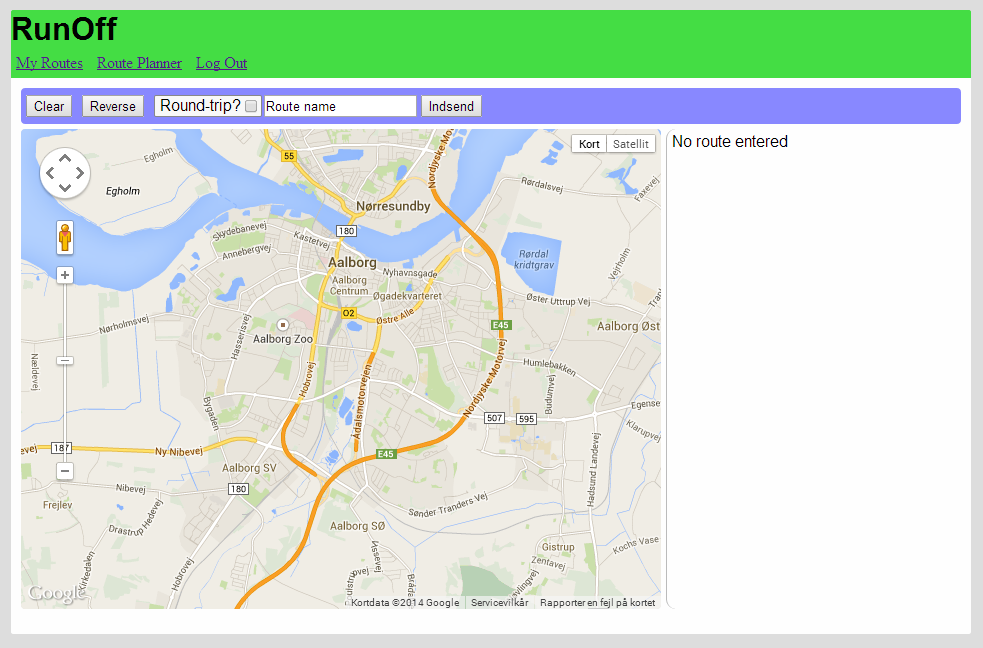
\includegraphics[width=\textwidth]{img/webplanner1.png}
\end{figure}

\subsection{Tests}
